%% APPENDIX B -- the spatial rank as a diagnostic: what it can and cannot
%% support, and the reserved hold-out that calibrates it.
%% Owner: r11-chain.  Carries \label{app:radius} (cited by 04_method.tex)
%% and \label{sec:heldout} (cited from the other appendices)
%% and \label{sec:nullscatter} (v4.23: cited by 05_results.tex's
%% false-alarm sentence, which quotes the MEASURED scatter of this very
%% null -- the reference used to read `app:spatialnorm`, a label that has
%% never existed in this tree and which stopped the build at `labelcheck`).
\section{The spatial rank, and what it can support}
\label{app:radius}

The spatial rank asks whether an excess sits at the star or anywhere else in
the field. It is a diagnostic, no disposition rests on it, and this appendix
is the measurement that settles why: \rankstatus{}

The star lies at the phase centre, inside the control annulus, and the
displacement is real: the star carries more above-threshold cells than a
control position at every level below the trigger. The chance expectation of
\S\ref{sec:trigunif} is not stepped by it, since the ratio at the trigger is
formed from the cells under test, and what it does when it is carried in is
measured once, in Appendix~\ref{app:falsealarm}. \emph{It is not a primary-beam effect.} Spectra are
extracted from phase-rotated visibilities in apparent flux density and are never
corrected for the primary-beam response (Appendix~\ref{app:conventions}), so
the familiar rise of image noise with distance from the pointing centre
cannot operate here; were it operating it would make the control probes
noisier than the star and place the stellar rank \emph{above} one half, the
opposite of what is measured. The control ensemble does show
a weak rise of its own level with radius, and each probe is therefore
standardised within its own radius bin, with no free parameter.

\emph{A calibration error that varied with frequency would explain the
displacement, and it is the only mechanism on offer.} An error identical in
every channel is removed exactly by the per-integration median along
frequency; a channel-dependent one is not, and two ordinary errors are
channel-dependent: a residual in the bandpass, and a system temperature
measured in the coarse correlator mode and interpolated onto the science
channels, which near a telluric line leaves a narrow feature behind
\citep{ALMATsys2018}. Both
multiply the continuum, so both act at the star and not on empty sky, both
stand still in topocentric frequency and both are coherent between
integrations: they would stack at near-zero drift and put the stellar rank
\emph{below} one half, the sign observed.
\emph{Amplitude excludes them, measured where the search looks.} Such an
error multiplies the continuum at the extraction position, a dirty-map
amplitude that includes any dust inside the synthesised beam; it must beat
the noise of the de-drifted, block-combined spectrum, since a
coherent residual stacks as a carrier does. A fractional error $\epsilon$
deposits $\epsilon S_{\rm c}$ at the star, so a crossing at the trigger needs
$\epsilon=5\sigma/S_{\rm c}$. That continuum is measured for each window in
its own execution block, as the time average of the window's own retained
spectra -- the same estimator as the search, at the same position -- over
\CyNWinMeas{} of the \CyNWinTot{} windows, and over \CyNRouteBlock{} blocks
it agrees with independent continuum images of
the same fields with no offset between the two (\CyRouteBiasMJy\,mJy).
No window in the survey requires as little as the
\CySpecTsysLo--\CySpecTsysHi{} per cent a coarse system temperature is
documented to leave at an ozone line: the smallest requirement anywhere is
\CyEpsMinPct{} per cent and the median \CyEpsMedPct, while over the
\CyNCrossMeas{} crossings with a measured continuum the least demanding
needs \CyCrossEpsLoPct{} per cent. The bandpass branch fails by amplitude
everywhere, needing
$\CyMarginBp\times$ the \CdSpecBpWorst{} per cent amplitude variation the
observatory quotes for its worst bands \citep{ALMAKBBandpass}, from the
bandpass stability campaign of \citet{ALMATechNote15}; and of either sample
\ScNInRad{} crossing lies within \ScRadMHz\,MHz -- two of the
\CdSpecTsysRes\,MHz channels on which the system temperature is measured --
of a catalogued atmospheric transition
(Appendix~\ref{app:rfi}), and it is counted as atmospheric. The shared noise
scale raises one further question, and the same arithmetic settles it: over
the \NsrNWin{} of
the \NWindows{} census windows that hold none of the adopted crossings, the
stellar statistic divided by the median of the \NCtrl{} control
statistics is exactly the ratio of the two noises; its median is \NsrMed{}
(\NsrLo--\NsrHi), so the two scales agree.

\subsection{The reserved hold-out, and what it calibrates}
\label{sec:heldout}

The statistic and the mask are set on the searched sample and cannot also
calibrate themselves, so a further sample is separated by an identifier rule:
a block is held out if and only if
$\mathrm{sha256}(\textsc{uid})_{[:8]} \bmod 5 = 0$, subject to two guards that
use identifiers alone -- a block on a named list stays in the
survey, and no system loses every block -- so that the assignment follows
from the UIDs and that list alone. That this sample is independent of the
choice of statistic and of mask is an assertion of ours and not something a
reader can check. Of
\NEbProcessedAll{} blocks processed, \NEbHeldOut{} are reserved, \HoPctHeld{}
per cent of them, carrying \HoWin{} windows toward \HoStars{} stars, with
no star and no system lost from the headline sample. The rule hashes the
execution block, and ALMA's identifier carries the observing session above
it, so \HsSharePct{} per cent of the reserved set -- \BkSessHoBlocks{} of
the \NEbHeldOut{} blocks, across \BkSessShared{} sessions -- shares
calibrators, weather and correlator setup with a searched block, where a
session-level hash would have been the stronger choice. Every quantity drawn
from this sample is therefore given twice, over the whole reserved set and
over the \HsIndBlocks{} blocks that share no session with it.
One further quantity is calibrated on those blocks and on nothing else, the
radial behaviour of the control ensemble: the standardised level
runs \HoRadBins{} across the annulus, a mean per-window slope of
$\HoRadSlope\pm\HoRadSlopeSe$, small and of the wrong sign to account for the
displacement.

\subsection{The recurrence statistic under the null}
\label{sec:nullscatter}

The exclusion in the crossing ledger is one formula. Writing $S$ and
$\sigma_{\rm d}$ for the discovery amplitude and its error, and $\bar{a}$ and
$\bar{\sigma}=(\sum_i\sigma_i^{-2})^{-1/2}$ for the inverse-variance
combination of the repeat readings at the predicted channel,
\begin{equation}
\sigma_{\rm excl}=\frac{S-\bar{a}}
{\sqrt{\sigma_{\rm d}^{2}+\bar{\sigma}^{2}}}
=\frac{T_{\rm pers}-T_{\rm rep}}{\sqrt{1+(T_{\rm pers}/T_\star)^{2}}},
\label{eq:excl}
\end{equation}
with $T_{\rm pers}=S/\bar{\sigma}$ and $T_{\rm rep}=\bar{a}/\bar{\sigma}$, so
every exclusion follows from three columns of that table and nothing else.
$T_{\rm rep}$ is read at the carried drift and at one cell; the largest value
over every drift trial at the same cell is tabulated beside it but is never
compared with $T_{\rm pers}$, since a maximum is positive on average whatever
is there. No exclusion can exceed the strength of the discovery it is built
from, nor is it the strongest statement available: an amplitude selected as
the largest of $10^{\TuCellsDecLo}$ to $10^{\TuCellsDecHi}$ cells at $T_\star\simeq5$ is biased high,
so a real carrier would be fainter than measured, and the
limit $(T_{\rm rep}+5)/T_{\rm pers}$ survives the bias, the
fraction of the discovery amplitude still ruled out at the trigger.

\emph{The same three numbers say where the test has power and where it has
none.} The criterion asks the repeat to reach the trigger, so a carrier
radiating through both observations at the discovery amplitude satisfies it
with probability $\Phi(T_{\rm pers}-5)$, and at the trigger amplitude
$5S/T_\star$ -- the faintest carrier that could have produced the crossing
at all -- with $\Phi(5T_{\rm pers}/T_\star-5)$. Where they are small the
crossing is untested and not excluded, and is reported that way.

\emph{That probability is calculated, and on every crossing that carries an
exclusion it is measured as well.} A
carrier at the trigger amplitude was injected at the predicted cell of every
covering repeat block through the instrument's own channel response, at a
sub-channel position drawn independently of the discovery's, into the
retained per-integration spectra of the discovery block and of every covering
repeat block -- \GpNRoleInj{} windows in all, before the baseline step, so
that the measurement is the recurrence reading -- and the readings combined
as the exclusion combines them, each realisation taking its noise
from a real reading of another channel of the same block. The accompanying
data give the measured recovery beside the calculated $\Phi$ for all
\HjNMeas: the rank-leading pair of \EvAStar{} and \EvBStar{} are recovered
\HjMeasSx{} and \HjMeasCp{} of the time over \HjMeasN{} realisations
apiece, against the \RqPowerTrigSx{} and \RqPowerTrigCp{} the expression
gives. Run with the
carrier amplitude set to zero the same harness returns each block's published
reading to the last digit, over \GpNullBlock{} readings of \GpNullStar{}
crossings. Over all \HjNMeas{} crossings that carry an exclusion the
experiment returns a median \HjDevMed{} less than the expression gives, and
two terms account for the difference: where in a channel the frame correction
places the carrier, which costs a median \HjRespMedPct{} per cent of the
amplitude, and the drift grid, which is sized to the discovery block, so that
carried into a repeat observation of a different length one of its steps
walks a different distance -- \HjEtaWalkCh{} channels in the one case where
the repeat is much the longer (\S\ref{sec:etacrv}), where the injection is
recovered \HjEtaMeas{} of the time against the one the expression gives.
A second harness built independently agrees to \HjCrossDev{} on the crossings
the two share, returning \RjMeasCp{} for \EvBStar{} where the two overlap;
the shortfall in the case just named is \HjDevMax, and the largest anywhere
else is \HjDevMaxOther{} at \HjDevStarOther. The \HjNPowerLo{} crossings
whose recovery chance is smallest
are the ones reported untested and not excluded, and every crossing's
recovery chance accompanies this paper as data, measured beside the
expression's own value.

\emph{The reading at the predicted channel is centred on zero and scatters
by one, measured and not merely designed.} Over \NuNullN{} single-cell
readings of every repeat block in the census and the hold-out its mean is
\NuNullMean{} and its scatter \NuNullSd. At the control positions of the
discovery windows it reads \NuDiscCtrlMean{} and \NuDiscCtrlSd. Over the
\WdBandNCross{} crossings scanned that way, the
largest value anywhere within $\pm$\WdBandKms\,km\,s$^{-1}$ of a predicted
channel is \WdBandMax{} at the carried drift; the
\RcTMax{} of Table~\ref{tab:cand} is its converse, one channel read at every
trial of the grid. A maximum behaves as a maximum
should: the largest of the
\NuCtrlRet{} retained control probes of a repeat block averages
\NuCtrlMean{} against \NuCtrlPred{} expected and the combined
$T_{\rm rep}$ of Eq.~\ref{eq:excl} averages \NuRepMean.
Widening the window
costs trials and not calibration: the repeat-epoch exceedances match the
same accounting, and the windows of \EcNShortStar{} stars are
narrower than the excursion an orbit at the grid ceiling could produce.

Figure~\ref{fig:bpiccontrol} draws both directions of the $\beta$~Pictoris
control, over the same \BpicPanelNDrawn{} of the \NCross{} crossings, the
remainder retaining no control ring. In its second panel the
\BpicPanelNCo{} $\beta$~Pictoris carbon-monoxide crossings land
\BpicDvCoLo--\BpicDvCoHi\,km\,s$^{-1}$ from CO in the star's own frame,
while the \BpicPanelNCs{} unattributed crossings of the same star have no
masked transition anywhere near them -- the nearest lies
\BpicDvCsLo--\BpicDvCsHi\,km\,s$^{-1}$ away -- and the methanol components
they do sit close to are excluded as their source in
Appendix~\ref{app:linemask}.

%% fig:bpiccontrol belongs here, where the spatial statistic is characterised.
\begin{figure}
\centering
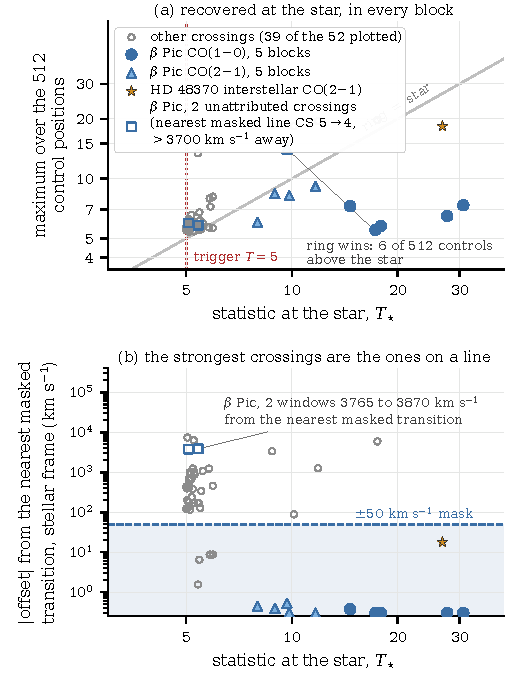
\includegraphics[width=\columnwidth]{figures/bpic_control.pdf}
%% ★★★ v4.26 (r25-captions): 16 PRINTED LINES -> R1 §7's limit of about six.
%% NINE macros had this caption as their only citation site.  Four --
%% \BpCtrlBlock, \BpCtrlBand, \BpCtrlRingMax, \BpCtrlStar -- went to
%% \S\ref{sec:bpicval}, into the sentence about the one block whose ring
%% beats the star, which described that block without naming it; the other
%% five -- \BpicPanelNDrawn, \BpicDvCoLo, \BpicPanelNCs, \BpicDvCsLo,
%% \BpicDvCsHi -- are the paragraph above, where this figure is introduced.
%% DELETED: the methanol offsets, which Appendix~\ref{app:linemask} states
%% in full and at greater length (\ZmOffLoMHz, \ZmOffHiMHz keep their sites
%% there), and "\NStageOneBpicEb{} of them with the star above every control"
%% which \S\ref{sec:bpicval} already carries.
\caption{The $\beta$~Pictoris positive control, in both directions
(\S\ref{sec:bpicval}). \emph{(a)}~The spatial screen: the stellar statistic
against the maximum over the window's \NCtrl{} control positions, filled for
the blocks recovering $\beta$~Pictoris CO. \emph{(b)}~Velocity offset from
the nearest masked transition \emph{in the star's own frame}, the adopted
$\pm\MaskHalfKms$\,km\,s$^{-1}$ half-width marked; grey, the
\BpicPanelNOther{} others, HD~48370 labelled.}
\label{fig:bpiccontrol}
\end{figure}
